\chapter{Basic Biological Computing in Python}
\label{chap:pythonI}

\epigraph{Science is what we understand well enough to explain to a 
computer. Art is everything else we do}{\textit{---Donald Knuth}}

{\bf Firstly, chapter \ref{chap:unix1}'s UNIX question?}
\begin{lstlisting}
find . -type f -exec ls -s {} \; | sort -n | head -10
\end{lstlisting}
What is the command doing? How has it been built (explain the components)?
% Sort and head to find the largest 10 files, including in 
% sub-directories. A faster option would be 
% find . -type f -exec ls -s {} + | sort -n | head -10
% See {\tt man find}, especially the part about the {\tt -exec option}

% Basically, -exec runs a command ({\tt ls -s} in this case) on each of 
% the files found, {} is replaced with the name of each file found, 
% and the find command is terminated by \;

\section{Outline of the {\tt python} module} 

The {\tt python} module is geared towards teaching you scientific 
programming in biology using this modern, and for good reason, 
immensely popular language. The components of this module across all 
the chapters (Basic, Advanced, Additional topics) are: 
\begin{compactitem}
	\item Basics of {\tt python}
	\item How to write and run {\tt python} code
	\item Understand and implement ``control flows''
	\item Learning to use the {\tt ipython} environment
	\item Writing, debugging, using, and testing {\tt python} functions
	\item Learning efficient numerical programming in {\tt python}
	\item Using regular expressions in {\tt python}  
	\item Introduction to certain particularly useful {\tt python} packages
	\item Using {\tt python} for building and modifying databases
	\item Using {\tt python} to run other ``stuff'' and to patch 
	together data analysis and/or numerical simulation work flows
\end{compactitem} 

\begin{figure} \centering
	    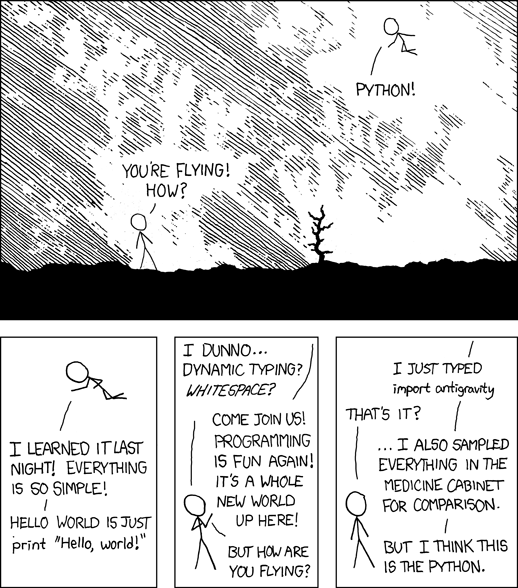
\includegraphics[width=.4\textwidth]{python.png}\\
		\url{www.xkcd.com}
	\caption{Is {\tt python} the most common answer to your daily 
	programming needs? Possibly!}
\end{figure}

\section{Why {\tt python}?}

{\tt python} was designed with readability and re-usability in mind. 
Time taken by programming + debugging + running is likely to be 
relatively lower in {\tt python} than less intuitive or cluttered 
languages (e.g., {\tt FORTRAN}, {\tt perl}). It is a pretty good 
solution if you want to  easily write readable code that is also 
reasonably efficient (computationally speaking).

\begin{figure}
	\begin{center}
    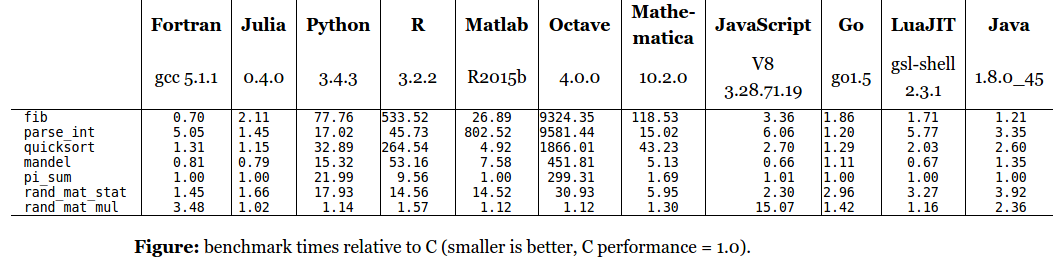
\includegraphics[width=1\textwidth]{benchmark.png}\\
		\url{http://julialang.org/}
	\end{center}
	\caption{{\tt python} is pretty fast!}
\end{figure}

\subsection{The Zen of python}
Open a terminal and type
\begin{lstlisting}
$ python -c "import this"
\end{lstlisting}

\section{Installing {\tt python}}

{\bf We will use 2.7.x, not 3.x (you can use 3.x later, if you want)}

Your Ubuntu distribution needs {\tt python}, so it will already be installed. 
However, let's install the interactive python shell {\tt ipython} which 
we will soon use.   
\begin{compactitem}[$\quad\star$]\itemsep4pt
\item On Ubuntu/Linux, open a terminal (ctrl+alt+t) and type:
\begin{lstlisting}
$ sudo apt-get install ipython python-scipy python-matplotlib
\end{lstlisting}
\end{compactitem}

\begin{tipbox}
In Linux, you can easily install python packages that come with the 
standard python distribution using the usual {\tt sudo apt-get install 
python-packagename}
\end{tipbox}
 
\section{Getting started with {\tt python}}
Open a terminal ({\tt ctrl+alt+t}) and type {\tt python} (or use the 
terminal that you just used to install {\tt ipython}). Then, try the 
following:
\begin{lstlisting}
>>> 2 + 2 # Summation; note that comments start with #
4

>>> 2 * 2 # Multiplication
4

>>> 2 / 2 # Integer division
1

>>> 2 / 2.0 # "Float" division, note the output is float
1.0

>>> 2 / 2.
1.0

>>> 2 > 3
False

>>> 2 >= 2
True
\end{lstlisting}

What does "float" mean in the above comment? Why is it necessary to 
specify this in Python (not necessary in Python 3.x)? You will 
inevitably run into some such jargon in this chapter. The main ones you 
need to know are (you will learn more about these along the way):

\begin{tabular}{p{2.2cm} p{12cm}} 
	Workspace & The state of the ``environment'' of your current python 
	{\it session}, including all variables, functions, objects, etc. \\ 
	Variable & A named number, text string, boolean ({\tt True} or {\tt False}), or data 
	structure that can change (more on variable	and data types later)\\
	Function &  A computer procedure or routine that returns some value(s), 
	and which can be used again and again \\
	Module & {\it Variables} and {\it functions} packaged into a single 
	set of programs that can be invoked as a command (potentially with sub-commands)  \\
	Class &  Also, variables and functions packaged into a single set of programs 
	that that can be invoked as a command (potentially with sub-commands), but unlike modules, you can spawn many 
	copies of a class within a python session or program\\
	Object & A particular instance of a class (every object belongs to a 
	class) that is created in  a session and eventually destroyed; 
	pretty much everything in your workspace is an object in python!  \\
\end{tabular}
This Module vs. Class vs. Object business is confusing. These 
constructs are created to make an (object-oriented) programming 
language like {\tt python} more flexible and user friendly (though it 
might not seem so to you currently!). In practice, at least for your 
current purposes, you will not build python classes yourself much, 
typically working with modules. More on all this later. Also, have a 
look at \url{https://learnpythonthehardway.org/book/ex40.html}

\subsection{\tt ipython}
We will now immediately switch to the {\tt i}nteractive {\tt python} 
shell, {\tt ipython} that you installed above. 

OK, now let's continue learning python using {\tt ipython}. 
\begin{compactitem}[$\quad\star$]\itemsep4pt{}
\item Type {\tt ctrl+D} in the terminal at the python prompt: this will 
exit you from the python shell and you will see the bash prompt again. 
\item Now type {\tt ipython}  
\end{compactitem}

You should now see (after some text):

\begin{lstlisting}
In [ ]: 
\end{lstlisting}
(I have deleted the prompt numbering {\tt [1]}, {\tt [2]}, etc to avoid 
confusion). This is the {\tt i}nteractive {\tt python} shell (or, "{\tt ipython}"). 
This shell has many advantages over the bare-bones, non-interactive 
python shell with the $>>>$ prompt. For example, as in the bash shell, 
{\tt TAB} leads to auto-completion of a command or file name (try it).

\subsection{Magic commands}
IPython also has ``magic commands'' (start with \%; e.g., {\tt \%run}). 
Some useful magic commands:

\begin{tabular}{p{2.5cm} p{10cm}} 
	{\tt \%who} & Shows current namespace (all variables, modules and 
	functions)\\
	{\tt \%whos} & Also display the type of each variable; typing {\tt 
	\%whos function} only displays functions etc.\\
  {\tt \%pwd} & Print working directory\\
	{\tt \%history} & Print recent commands\\
\end{tabular}

Try any of these now!
 
\subsection{Determining an object's type}
Another useful IPython feature is the question mark, which can be used 
to find what a particular Python object is, including variables you 
created. For example, try: 
\begin{lstlisting}
In [1]: a = 1

In [2]: ?a
Type:        int
String form: 1
Docstring:
int(x=0) -> int or long
int(x, base=10) -> int or long

Convert a number or string to an integer, or return 0 if no arguments
are given.  If x is floating point, the conversion truncates towards zero.
If x is outside the integer range, the function returns a long instead.

If x is not a number or if base is given, then x must be a string or
Unicode object representing an integer literal in the given base.  The
literal can be preceded by '+' or '-' and be surrounded by whitespace.
The base defaults to 10.  Valid bases are 0 and 2-36.  Base 0 means to
interpret the base from the string as an integer literal.
>>> int('0b100', base=0)
4
\end{lstlisting}

\begin{tipbox}
You can configure ipython's environment and behavior by editing 
the {\tt ipython\_config.py} file:
\begin{lstlisting}
$ geany ~/.config/ipython/profile_default/ipython_config.py &
\end{lstlisting}
This file does not inititally exist, but you can create it by running  
{\tt ipython profile create} in a bash terminal (try it now). 

Now you can configure ipython. For example, If you don't like the blue 
{\tt ipython} prompt, you can type {\tt \%colors linux} (once inside 
the shell). If you want to make this color the default, then edit {\tt 
ipython\_config.py} --- search for ``Set the color scheme'' in the 
file. 
\end{tipbox}
\section{Python variables}

Now, let's continue our python intro. We will first learn about the {\tt 
python} variable types that were mentioned above. The types are:

\begin{lstlisting}
In [ ]: a = 2 #integer

In [ ]: ?a
Type:        int
String form: 2
Docstring:
int(x=0) -> int or long
int(x, base=10) -> int or long

Convert a number or string to an integer, or return 0 if no arguments
are given.  If x is floating point, the conversion truncates towards zero.
If x is outside the integer range, the function returns a long instead.

If x is not a number or if base is given, then x must be a string or
Unicode object representing an integer literal in the given base.  The
literal can be preceded by '+' or '-' and be surrounded by whitespace.
The base defaults to 10.  Valid bases are 0 and 2-36.  Base 0 means to
interpret the base from the string as an integer literal.
>>> int('0b100', base=0)
4

In [ ]: a = 2. #Float

In [ ]: ?a
Type:        float
String form: 2.0
Docstring:
float(x) -> floating point number

Convert a string or number to a floating point number, if possible.

In [ ]: a = "Two" #String

In [ ]: ?a
Type:        str
String form: Two
Length:      3
Docstring:
str(object='') -> string

Return a nice string representation of the object.
If the argument is a string, the return value is the same object.

In [10]: a = True #Boolean

In [11]: ?a
Type:        bool
String form: True
Docstring:
bool(x) -> bool

Returns True when the argument x is true, False otherwise.
The builtins True and False are the only two instances of the class bool.
The class bool is a subclass of the class int, and cannot be subclassed.
\end{lstlisting}

Thus, {\tt python} has integer, float (real numbers, with different 
precision levels) and string variables.

\subsection{{\tt python} operators}
Here are are the operators in python that you can use on variables:

\begin{tabular}{p{2cm} p{10cm}} 
  {\tt +} & Addition\\
  {\tt -} & Subtraction\\
  {\tt *} & Multiplication\\
  {\tt /} & Division\\
  {\tt **} & Power\\
  {\tt \%} & Modulo\\
  {\tt //} & Integer division\\
  {\tt ==} & Equals\\
  {\tt !=} & Differs\\
  {\tt $>$} & Greater\\
  {\tt $>$=} & Greater or equal\\
  {\tt \&, and} & Logical and\\
  {\tt $\vert$, or} & Logical or\\
  {\tt !, not} & Logical not\\	
\end{tabular}

\subsection{Assigning and manipulating variables}

\begin{lstlisting}
 In []: 2 == 2
Out []: True

 In []: 2 != 2
Out []: False

 In []: 3 / 2
Out []: 1

 In []: 3 / 2.
Out []: 1.5

 In []: 'hola, ' + 'mi llamo Samraat' #why not two languages at the same
time?! 
Out []: 'hola, mi llamo Samraat'

In []: x = 5

 In []: x + 3
Out []: 8

 In []: y = 8

 In []: x + y
Out []: 13

 In []: x = 'My string'

 In []: x + ' now has more stuff'
Out []: 'My string now has more stuff'

 In []: x + y
Out []: TypeError: cannot concatenate 'str' and 'int' objects
\end{lstlisting}

OK, so concatenating string and numeric (integer in this case) 
variables doesn't work.  No problem, we can convert from one type to 
another:

\begin{lstlisting}
 In []: x + str(y)
Out []: 'My string8'

 In []: z = '88'

 In []: x + z
Out []: 'My string88'

 In []: y + int(z)
Out []: 96
 \end{lstlisting} 

\begin{tipbox}
In {\tt python}, the type of a variable is determined when the  program 
or command is running (dynamic typing) (like {\tt R}, unlike {\tt C} or 
{\tt FORTRAN}). This is convenient, but can make programs slow. More 
on efficient computing later.
\end{tipbox}

\section{{\tt python} data types and data structures}

{\tt python} number or string variables (or both) can be stored and manipulated in:
\begin{compactitem} \itemsep4pt
 \item  {\bf List}: most versatile, can contain compound data, ``mutable'',
enclosed in brackets, [ ]
 \item  {\bf Tuple}: like a list, but ``immutable'' --- like a read only list,
enclosed in parentheses,  ( ) 
 \item  {\bf Dictionary}: a kind of ``hash table'' of key-value pairs enclosed
by curly braces, \{ \} --- key can be number or string, values can be any
object! (well OK, a python object)
 \item  {\bf numpy arrays}: Fast, compact, convenient for numerical computing --- more on this later!
\end{compactitem}

\subsection{Lists}

\begin{lstlisting} 
 In []: MyList = [3,2.44,'green',True]

 In []: MyList[1]
Out []: 2.44

 In []: MyList[0] # NOTE: FIRST ELEMENT -> 0
Out []: 3

 In []: MyList[4]
Out []: IndexError: list index out of range

 In []: MyList[2] = 'blue'

 In []: MyList
Out []: [3, 2.44, 'blue', True]

 In []: MyList[0] = 'blue'

 In []: MyList
Out []: ['blue', 2.44, 'blue', True]

 In []: MyList.append('a new item') # NOTE: ".append"!

 In []: MyList
Out []: ['blue', 2.44, 'blue', True, 'a new item']

 In []: MyList.sort() # NOTE: suffix a ".", hit tab, and wonder!

 In []: MyList
Out []: [True, 2.44, 'a new item', 'blue', 'blue']
\end{lstlisting}

In the above commands, notice that {\tt python} "indexing" starts at 0, 
not 1!  

\subsection{Tuples}

\begin{lstlisting} 
 In []: FoodWeb=[('a','b'),('a','c'),('b','c'),('c','c')]

 In []: FoodWeb[0]
Out []: ('a', 'b')

 In []: FoodWeb[0][0]
Out []: 'a'

 In []: FoodWeb[0][0] = "bbb"  # NOTE: tuples are "immutable"
      TypeError: 'tuple' object does not support item assignment

 In []: FoodWeb[0] = ("bbb","ccc")

 In []: FoodWeb[0]
Out []: ('bbb', 'ccc')
\end{lstlisting} 

Note that tuples are "immutable"; that is, a particular pair or 
sequence of strings or numbers cannot be modified after it is created.

In the above example, why assign these food web data to a list of 
tuples and not a list of lists? --- because we want to maintain the 
species associations, no matter what --- they are sacrosanct! 

Tuples contain immutable sequences, but you can append to them:

\begin{lstlisting} 
 In []: a = (1, 2, [])
 
 In []: a[2].append(1000)
 
 In []: a
Out []: (1, 2, [1000])
\end{lstlisting}

\subsection{Sets}
You can convert a list to an immutable ``set'' --- an unordered 
collection with no duplicate elements. Once you create a set you
can perform set operations on it:

\begin{lstlisting} 
 In []: a = [5,6,7,7,7,8,9,9]

 In []: b = set(a)

 In []: b
Out []: set([8, 9, 5, 6, 7])

 In []: c = set([3,4,5,6])

 In []: b & c
Out []: set([5, 6])

 In []: b | c
Out []: set([3, 4, 5, 6, 7, 8, 9])

 In []: list(b | c) # set to list
Out []: [3, 4, 5, 6, 7, 8, 9]

\end{lstlisting}

The key set operations in {\tt python} are: 

\begin{tabular}{p{2.5cm} p{10cm}} 
	{\tt a - b } & a.difference(b)\\
	{\tt a $<=$ b} & a.issubset(b)\\
	{\tt a $>=$ b} & b.issubset(a)\\
	{\tt a \& b} & a.intersection(b)\\
	{\tt a $\vert$ b} & a.union(b)\\
\end{tabular}

\subsection{Dictionaries}

A set of values (any {\tt python} object) indexed by keys (string or 
number), a bit like {\tt R} lists.

\begin{lstlisting} 
In []: GenomeSize = {'Homo sapiens': 3200.0, 'Escherichia coli': 4.6,
'Arabidopsis thaliana': 157.0}

 In []: GenomeSize
Out []: 
{'Arabidopsis thaliana': 157.0,
  'Escherichia coli': 4.6,
  'Homo sapiens': 3200.0}

 In []: GenomeSize['Arabidopsis thaliana']
Out []: 157.0

 In []: GenomeSize['Saccharomyces cerevisiae'] = 12.1

 In []: GenomeSize
Out []: 
{'Arabidopsis thaliana': 157.0,
'Escherichia coli': 4.6,
'Homo sapiens': 3200.0,
'Saccharomyces cerevisiae': 12.1}

 In []: GenomeSize['Escherichia coli'] = 4.6  # ALREADY IN DICTIONARY!

 In []: GenomeSize
Out []: 
{'Arabidopsis thaliana': 157.0,
 'Escherichia coli': 4.6,
 'Homo sapiens': 3200.0,
 'Saccharomyces cerevisiae': 12.1}

 In []: GenomeSize['Homo sapiens'] = 3201.1

 In []: GenomeSize
Out []: 
{'Arabidopsis thaliana': 157.0,
 'Escherichia coli': 4.6,
 'Homo sapiens': 3201.1,
 'Saccharomyces cerevisiae': 12.1} 
\end{lstlisting}

So, in summary, 
\begin{compactitem} \itemsep10pt
	\item  If your elements/data are unordered and indexed by numbers use 
	{\bf lists}
  \item  If they are ordered sequences use a {\bf tuple} 
	\item  If you want to perform set operations on them, use a {\bf set}
	\item  If they are unordered and indexed by keys (e.g., names), use a 
	{\bf dictionary}
\end{compactitem}

{\it But why not use dictionaries for everything?} -- because it can 
slow down your code!

\subsection{Copying mutable objects}

Copying mutable objects can be tricky. Try this:

\lstinputlisting{Practicals/Code/deepcopy.py}

So, you need to employ {\tt deepcopy} to really copy an existing object 
or variable and assign a new name to the copy. 

\begin{tipbox}
	Python does shallow copying of mutable objects for computing performance considerations. By not copying the underlaying object when you re-assign a mutable object to a new ("variable") name, Python avoids unnecessary memory copying ("passing by reference"). That does nit change the fact that shallow vs. deep copying can be confusing, of course!
\end{tipbox} 

\subsection{{\tt python} with strings}

One of the things that makes python so useful and versatile, is that it 
has a powerful set of inbuilt commands to perform string manipulations. 
For example, try these: 

\lstinputlisting{Practicals/Code/exstrings.py}

\section{Writing {\tt python} code}

Now let's learn to write and run python code from a {\tt *.py} file. 
But first, some some guidelines for good code-writing practices (see
\url{python.org/dev/peps/pep-0008/}):
  \begin{compactitem} \itemsep8pt
    \item Wrap lines to be $<$80 characters long. You can use parentheses $()$
  or signal that the line continues using a ``backslash'' $\backslash$
    \item Use either 4 spaces for indentation or tabs, but not both! (I use tabs!)
    \item Separate functions using a blank line
    \item When possible, write comments on separate lines
  \end{compactitem}

Make sure you have chosen a particular indent type (space or tab) in 
{\tt geany} (or whatever IDE you are using) --- indentation is all-important 
in {\tt python}. Furthermore, 
\begin{compactitem} \itemsep4pt
    \item Use ``docstrings'' to {\bf document how to use the code}, and
      {\bf comments to explain why and how the code works}
    \item Naming conventions (bit of a mess, you'll learn as you go!):
    \begin{compactitem}
      \item {\tt \_internal\_global\_variable} (for use inside module only)
      \item {\tt a\_variable}
      \item {\tt SOME\_CONSTANT}
      \item {\tt a\_function}
			\item Never call a variable {\tt l} or {\tt O} or {\tt o}\\ {\it 
			why not?} -- you are likely to confuse it with {\tt 1} or {\tt 0}!
    \end{compactitem}
	\item Use spaces around operators and after commas:\\ 
  {\tt  a = func(x, y) + other(3, 4)} 
\end{compactitem}

\section{{\tt python} Input/Output}

Let's look at importing and exporting data.  Make a textfile called 
{\tt test.txt} in {\tt Week2/Sandbox/} with the following content 
(including the empty lines):

\begin{lstlisting}
First Line
Second Line

Third Line

Fourth Line
\end{lstlisting}

Then, type the following in {\tt Week2/Code/basic\_io.py} (note the 
indentation!):

\lstinputlisting{Practicals/Code/basic_io.py}

Note the following:

\begin{compactitem}
	\item The {\tt for line in f} is an implicit loop --- implicit 
	because stating the range of things in {\tt f} to loop over in this 
	way allows python to handle any kind of objects to loop thorugh. For 
	example, if {\tt f} was an array of numbers 1 to 10, it would loop 
	thorugh them; if {\tt f} is a file, as in the case of the script 
	above, it will loop through the lines in the file.
	
	\item {\tt is len(line.strip()) > 0} checks if the line is empty. Try 
	{\tt ?} to see what {\tt .strip()} does.	 
\end{compactitem}

The {\tt csv} package makes it easy to manipulate CSV files (get {\tt 
testcsv.csv} from {\tt CMEEMasteRepo}). Type the following script in 
{\tt Week2/Code/basic\_csv.py}
  
\lstinputlisting{Practicals/Code/basic_csv.py}

\begin{tipbox}
Now that you have seen how all-important indentation of python code is, 
you might find the {\tt ipython \%cpaste} function very handy, as it 
allows you to run fragments of code, indentation and all, directly in 
the {\tt ipython} commandline. Let's try it. Type the following code 
in a temporary file:
\begin{lstlisting}
for i in range(x):
		if i > 3: #4 spaces or 2 tabs in this case
				print i 
\end{lstlisting}
Now, assign some integer value to a variable {\tt x}: 
\begin{lstlisting}
In [ ]: x = 11
\end{lstlisting}
Then,
\begin{lstlisting}
In [ ]: %cpaste
Pasting code; enter '--' alone on the line to stop or use Ctrl-D.
:for i in range(x):
:    if i > 3: #4 spaces or 2 tabs in this case
:        print i
:--
4
5
6
7
8
9
10
\end{lstlisting}
Of course, this code is simple, so directly pasting works as well --- 
{\tt \%cpaste} is really useful when you have more complex code fragments 
you want to try out. Se haow far you have to pus direct pasting till 
you need {\tt \%cpaste}
\end{tipbox}

\subsection{Writing {\tt python} functions (or modules)}

Now let's writing proper {\tt python} functions. We will start with a 
``boilerplate'' code. Type the code below and save as {\tt 
boilerplate.py} in {\tt CMEECourseWork/Week2/Code}:

\lstinputlisting{Practicals/Code/boilerplate.py}

\subsubsection{Running your {\tt python} code}

Now {\tt cd } to the directory and run the code:
\begin{lstlisting}
$ cd ~/Documents/../CMEECourseWork/Week2/Code
$ python boilerplate.py
\end{lstlisting}

You should see "This is a boilerplate" in your terminal window. 

Alternatively, you can use ipython:
\begin{lstlisting} 
$ ipython boilerplate.py
\end{lstlisting}

You can also execute a python script file from within the {\tt ipython} 
shell with {\tt run MyScript.py}. So, enter {\tt ipython} from bash, 
and do: 
\begin{lstlisting} 
In [ ]: run boilerplate.py
\end{lstlisting}

To run the script from the native python shell, you would use {\tt 
execfile("MyScript.py")}.

\subsection{Components of the {\tt python} function}

Now let's look at the elements of your first, boilerplate code:

\subsubsection{The shebang}

Just like UNIX shell scripts, the first "shebang" line tells the 
computer where to look for python. It determines the script's ability 
to be executed like an standalone executable without typing python 
beforehand in the terminal or when double clicking it in a file 
manager (when configured properly to be an executable). It isn't 
necessary but generally put there so when someone sees the file opened 
in an editor, they immediately know what they're looking at. However, 
which shebang line you use is important. 

Here by using {\tt \#!/usr/bin/python} we are specifying the location 
to the python executable in your machine that rest of the script needs 
to be interpreted with. You may want to use {\tt \#!/usr/bin/env 
python} instead, which will prevent failure to run if the Python 
executable on some other machine or distribution isn't actually located 
at {\tt \#!/usr/bin/python}, but elsewhere.

\subsubsection{The Docstring}

Triple quotes start a ``docstring'' comment, which is meant to describe 
the operation of the script or a function/module within it. docstrings 
are considered part of the running code, while normal comments are 
stripped. Hence, you can access your docstrings at run time. It is a 
good idea to have doctrings at the start of every python script and 
module as it can provide useful information to the user and you as 
well, down the line. 

You can access the docstring(s) in a script (both 
for the overall script and the ones in each of its functions), by 
importing the function (say, {\tt my\_func}), and then typing {\tt 
help(my\_func)} in the python or ipython shell. For example, try {\tt 
import boilerplate} and then {\tt help(boilerplate)} (but you have 
to be in the python or ipython shell). 

For more info, see \url{https://www.python.org/dev/peps/pep-0257}

\subsubsection{Internal Variables}

%% What's going on here?
``{\tt \_\_}'' signal ``internal'' variables (never name your
variables so!)

\subsubsection{Function {\tt def}initions and "modules"}

{\tt def} indicates the start of a python function; all subsequent 
lines must be indented.

It's important to know that somewhat confusingly, Pythonistas 
call a file containing function {\tt def}itions's) and statements 
(e.g., assignments of constant variables) a "module". There is a 
practical reason (there's always one!) for this. You might want to use 
a particular set of python {\tt def}'s (functions) and statements 
either as a standalone function, or use it or subsets of it from other 
scripts. So in theory, every function you {\tt def}ine can be a 
sub-module usable by other scripts. 

{\it In other words, {\tt def}initions from a module can be imported 
into other modules and scripts, or into the main module itself.} 

At this juncture, you might also want to know more about a Python 
"class". Have a look at 
\url{http://learnpythonthehardway.org/book/ex40.html} --- a nice, 
intuitive tutorial that should help you understand functions vs. 
modules vs. classes in Python.

The last few lines, including the {\tt main} function/module are 
somewhat esoteric but important; more on this below.
 
\subsubsection{Why include {\tt \_\_name\_\_ == "\_\_main\_\_"} and all 
that jazz}

When you run a Python module with or without arguments, the code in the 
called module will be executed just as if you imported it, but with the 
{\tt \_\_name\_\_} set to {\tt "\_\_main\_\_"}. So adding this code 
at the end of your module,
\begin{lstlisting}
if (__name__ == "__main__"):
\end{lstlisting}
directs the {\tt python} interpreter to set the special {\tt 
\_\_name\_\_} variable to have a value "{\tt  \_\_main\_\_}", so that 
the file is usable as a script as well as an importable module. How do 
you import? Simply as (in python or ipython shell):
\begin{lstlisting}
In []: import boilerplate
\end{lstlisting}
Then type 
\begin{lstlisting}
In []: boilerplate
Out[]: <module 'boilerplate' from 'boilerplate.py'>
\end{lstlisting}

One more script to hopefully clarify this further. Type and save the 
following in a script file called {\tt using\_name.py}: 
\lstinputlisting{Practicals/Code/using_name.py}
Now run it:
\begin{lstlisting}
In []: run using_name.py
This program is being run by itself
\end{lstlisting}

Now, try:
\begin{lstlisting}
In []: import using_name
I am being imported from another module
\end{lstlisting}
	
The output {\tt I am being imported from another module} will only 
show up once. 

Also please look up \url{https://docs.python.org/2/tutorial/modules.html}

\subsubsection{What on earth is {\tt sys.argv}?}

In your boilerplate code, as any other Python code, {\tt argv} is the 
"argument variable". Such variables are necessarily very common across 
programming languages, and play an important role --- {\tt argv} is a 
variable that holds the arguments you pass to your Python script when 
you run it. {\tt sys.argv} is simply an object created by python 
using the {\tt sys} module (which you imported at the beginning of the 
script) that contains the names of the argument variables in the 
current script.

To understand this in a practical way, let's write and save 
a script called {\tt sysargv.py}: 
\lstinputlisting{Practicals/Code/sysargv.py}
Now run {\tt sysargv.py} with different numbers of arguments:
\begin{lstlisting}
run sysargv.py
run sysargv.py var1 var2
run sysargv.py 1 2 var3
\end{lstlisting}
As you can see the first variable is always the file name, and is always 
available as to the Python interpreter.

Then, the command {\tt main(argv=sys.argv)} directs the interpreter to 
pass the argument variables to the main function. Which brings us to,
\begin{lstlisting}
def main(argv):
    print 'This is a boilerplate' # NOTE: indented using two tabs or four spaces
\end{lstlisting}
This is the main function. Arguments obtained in the {\tt if 
(\_\_name\_\_ == "\_\_main\_\_"):} part of the script are "fed" to this 
main function where the printing of the line "This is a boilerplate" 
happens.

OK, finally, what about this bit: 
\begin{lstlisting}
sys.exit(status) 
\end{lstlisting}

It's just a way to terminate and exit the Python program in an explicit 
manner, returning an appropriate status code. In this case, we have 
decided that {\tt main()} returns 0 on a successful run, so {\tt 
sys.exit(status)} will return zero indicating ``successful 
termination''. Try putting {\tt sys.exit("I am exiting right now!") } 
in other places in {\tt boilerplate.py} and see what happens.  

\subsection{Variable scope}

One important thing to note about functions, in any language, is that 
variables inside functions are invisible outside of it, nor do they 
persist once the function has run. These are called "local" variables, 
and are only accessible inside their function. However, "global" 
variables are visible inside and outside of functions. In python, you 
can assign global variables. Type the following script in {\tt 
scope.py} and try it:
  
\lstinputlisting{Practicals/Code/scope.py}

However, in general, avoid assigning globals because you run the risk 
of "exposing" unwanted variables to all functions within your name 
work/namespace. 

\section{Control statements}

OK, let's get deeper into {\tt python} functions. To begin, first copy 
and rename {\tt boilerplate.py} (to make use of it's existing 
structure and save you some typing):
\begin{lstlisting}  
$ cp boilerplate.py control_flow.py
$
\end{lstlisting}
Then type the following script into {\tt control\_flow.py}:
\lstinputlisting{Practicals/Code/control_flow.py}

Now run the code:
\begin{lstlisting}
In []: run control_flow.py
\end{lstlisting}

You can also call any of the functions within {\tt control\_flow.py}:
\begin{lstlisting}
In []: even_or_odd(11)
Out[]: '11 is Odd!'
\end{lstlisting}
This is possible without explicitly importing the modules because you 
are only running one script. You would have to do an explicit {\tt 
import} if you needed a module from another python script file.

\subsection{Control flow exercises}

\begin{compactitem} [$\quad\star$]\itemsep4pt
	\item Write the following, and save them to {\tt cfexercises.py}.
	\item Now try these {\it function by function}, pasting the block in 
	the ipython command line (hopefully you have set youe code editor to 
	send a selection to the commandline by now) 

\end{compactitem}

\lstinputlisting{Practicals/Code/cfexercises.py}

\section{Loops}

Write the following, and save them to {\tt loops.py}.
\lstinputlisting{Practicals/Code/loops.py}
\begin{figure}
	\begin{center}
    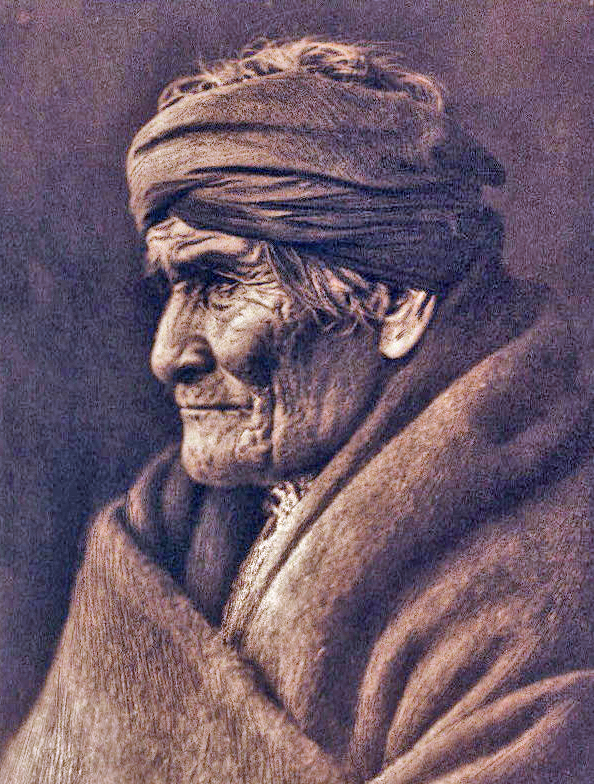
\includegraphics[width=.5\textwidth]{Geronimo.jpg}
\end{center}
\caption{In case you were wondering who Geronimo was.}
\end{figure}

\subsection{List comprehensions}

Python offers a way to combine loops, functions and logical tests in a 
single line of code. Type the following in a script file called {\tt 
oaks.py}:

\lstinputlisting{Practicals/Code/oaks.py}

Don't go mad with list comprehensions --- code readability is more 
important than squeezing lots into a single line! 

\section{Practicals}
As always, test, add, commit and push all your new code and data to 
your git repository. 

\begin{enumerate}

	\item Modify {\tt cfexercises.py} to make it a ``module'' like {\tt 
	control\_flow.py}). That is, all the {\tt fooXX} functions should 
	take arguments from the user (like the functions inside {\tt 
	control\_flow.py}. Also, add some test arguments to show that they 
	work (again, like {\tt control\_flow.py}) --- for example, 
	"foo5(10)". Thus, running {\tt cfexercises.py} should now also output 
	evaluations of all the {\tt fooXX} modules along with a bunch of 
	hellos.

	\item Open and complete the tasks in {\tt lc1.py}, 
	{\tt lc2.py}, {\tt dictionary.py}, {\tt tuple.py} (you can tackle 
	them in any order) 

\end{enumerate}

\section{Functions, Modules, and code compartmentalization}
 
 Ideally you should aim to compartmentalize your code into a bunch of 
 functions, typically written in a single {\tt .py} file: this are  
 Python ``modules'', which you were introduced to previously. Why bother 
 with modules? Because:

\begin{compactitem}
 
	\item Keeping code compartmentalized  is good for debugging, unit
  testing, and profiling (coming up later)
	\item Makes code more compact by minimizing redundancies (write
  repeatedly used code segments as a module)
	\item Allows you to import and use useful functions that you yourself
wrote, just like you would from standard python packages (coming up)
      \end{compactitem}

\subsection{Importing Modules}

There are different ways to {\bf import} a module:
\begin{compactitem}
  \item {\tt import my\_module}, then functions in the module can be called
as \\ {\tt my\_module.one\_of\_my\_functions()}.
  \item {\tt from my\_module import my\_function} imports only the
function {\tt my\_function} in the module {\tt my\_module}. It can then be
called as if it were part of the main file: {\tt my\_function()}.
  \item {\tt import my\_module as mm} imports the module
    {\tt my\_module} and calls it {\tt mm}. Convenient when the name of
the module is very long. The functions in the module can be called as
    {\tt mm.one\_of\_my\_functions()}.
  \item {\tt from my\_module import *}. Avoid doing this! \\ 
  {\it Why?} -- to avoid name conflicts!

  \item You can also access variables written into modules: {\tt import
my\_module}, then \\ {\tt my\_module.one\_of\_my\_variables}
\end{compactitem}

\section{Python packages}

A Python package is simply a directory of Python modules (quite like an 
{\tt R} package). Many packages, such as the following that I find 
particularly useful, are always available as standard libraries (just 
require {\tt import} from within python or ipython):

\begin{compactitem}
	\item {\tt io}: file input-output with {\tt *.csv}, {\tt *.txt}, etc.
	\item {\tt subprocess}: to run other programs, including multiple ones
at the same time, including operating system-dependent functionality 
	\item {\tt sqlite3}: for manipulating and querying {\tt sqlite}
databases
	\item {\tt math}: for mathematical functions
\end{compactitem}

Scores of other packages are accessible by explicitly installing them 
using \\{\tt sudo apt-get install python-packagename} (as you did 
previously) or by using {\tt pip}. Some particularly mentionable ones are:

\begin{compactitem}
		\item {\tt sciPy} (\url{http://scipy.org}) contains a wide array of numerical 
		tools  for scientific computing, including {\tt NumPy} for efficient data crunching
		\item {\tt matplotlib}: for plotting (very matlab-like, requires 
	 {\tt scipy}) (all packaged in {\tt pylab})
		\item {\tt pandas} provides a powerful set of methods to 
		manipulating data, and comes with a DataFrame object similar to the
		{\tt R} data frame.
		\item {\tt scikit-learn} \url{http://scikit-learn.org/} for applying 
		different machine learning algorithms to data
		\item {\tt ipython} an enhanced python terminal (which we are 
		currently using!) 
		\item {\tt jupyter} an interactive notebook environment for 
		exploratory data analysis, visulaization, and creation of interactive 
	 documents that can be shared. This course is in the process of being written entirely in Jupyter notebooks.
	 \item {\tt scrapy}: for writing web spiders that crawl web sites and 
	 extract data from them
	 \item {\tt beautifulsoup}: for parsing HTML and XML (can do what 
	 {\tt scrapy} does)
	 \item {\tt biopython}: for bioinformatics
\end{compactitem}
Of course, you have already installed some of these ({\tt scipy}, {\tt 
matplotlib}). 

For those of you interested in bioinformatics, the {\tt biopython} 
package will be particularly useful. We will not cover bioinformatics 
in any depth within the python weeks, but you may want to try 
to use Python for bioinformatics in other weeks, especially the 
Genomics weeks, and perhaps use it for your own research projects. I suggest that if bioinformatics is your thing, check out 
{\tt biopython} --- in particular the worked examples at 
\url{http://biopython.org/DIST/docs/tutorial/Tutorial.html}.


\section{Practicals}
As always, test, add, commit and push all your new code and data to 
your git repository. 

\subsubsection{Align DNA sequences}

Align two DNA sequences such that they are as similar as possible. 

The idea is to start with the longest string and try to position the 
shorter string in all possible positions. For each position, count a 
``score'' : number of bases matched perfectly over the number of bases 
attempted. Your tasks:

 \begin{enumerate} \itemsep3pt
 
		\item Open and run {\tt Practicals/Code/align\_seqs.py} --- make 
		sure you understand what each line is doing to do this)

		Now convert {\tt align\_seqs.py} to a Python function that 
		takes the DNA sequences as an input from a single external file and 
		saves the best alignment along with its corresponding score in a 
		single text file (your choice of format and file type) to an 
		appropriate location. No external should be needed; that is, you 
		should still only need to use {\tt python align\_seq.py} to run it. 
		
		For example, the input file can be a single {\tt .csv} file 
		with the two example sequences given at the top of the original 
		script.

		{\it Don't forget to add docstrings where necessary/appropriate.} 

		\item Extra Credit -- align all the {\tt .fasta} sequences from 
		Week 1; call the new script \\ {\tt align\_seqs\_fasta.py}. Unlike 
		align\_seqs.py, this script should take {\it any} two fasta sequences (in 
		separate files) to be aligned as input. So this script would 
		typically run by using explicit inputs, by calling something like {\tt python 
		align\_seqs\_fasta.py seq1.csv seq2.csv}. However, it should 
		still run if no inputs were given, using two fasta sequences  
		from {\tt Data} as defaults.

  \end{enumerate}

\section{Errors in your {\tt python} code}

What do you want from your code? Rank the following by importance:
  \begin{enumerate}
    \item it is very fast
    \item it gives me the right answer
    % \item it is possible to test it
    % \item it has lots of tests
    \item it is easy to read
    \item it uses lots of 'clever' programming techniques
    \item it uses cool features of the language
  \end{enumerate}

Then, think about this: 

  \begin{compactitem}
     \item If you are {\it very lucky}, your program will crash when you run it
     \item If you are {\it lucky}, you will get an answer that is obviously wrong
     \item If you are {\it unlucky}, you won't notice until after publication
     \item If you are {\it very unlucky}, someone else will notice it after 
publication
  \end{compactitem}
  
Ultimately, most of your time could well be spent error-checking and 
fixing them ``debugging'', not writing code. You can debug when errors 
appear, but why not just nip as many as you can in the bud? For this, 
you would use unit testing.

\subsection{Unit testing}

Unit testing prevents the most common mistakes and helps write reliable 
code. Indeed, there are many reasons for testing:
\begin{compactitem}
	\item Can you prove (to yourself) that your code does what you think it does?
	\item Did you think about the things that might go wrong?
	\item Can you prove to other people that your code works?
	\item Does it still all work if you fix a bug?
	\item Does it still all work if you add a feature?
	\item Does it work with that new dataset?
	\item Does it work on the latest version of the language (e.g., 
	Python 3.x vs.\ 2.7.x)?
	\item Does it work on Mac? on Linux? on Windows?
	\item Does it work on 64 bit {\it and} 32 bit?
	\item Does it work on an old version of a Mac?
	\item Does it work on Harvey, or Imperial's Linux cluster?
\end{compactitem}

The idea is to write \textit{independent} tests for the {\it smallest 
units} of code. Why the smallest units? --- to be able to retain the 
tests upon code modification. 

\subsubsection{Unit testing with {\tt doctest}}

Let's try {\tt doctest}, the simplest  testing tool in python: 
simpletests for each function are  embedded in the docstring. Copy the 
file {\tt control\_flow.py} into the file {\tt test\_control\_flow.py} 
and edit the original function so:

\lstinputlisting{Practicals/Code/test_control_flow.py}

Now type {\tt  run test\_control\_flow.py -v} :
  
\begin{lstlisting}
In []: run  test_control_flow.py -v
Trying:
    even_or_odd(10)
Expecting:
    '10 is Even!'
ok
Trying:
    even_or_odd(5)
Expecting:
    '5 is Odd!'
ok
Trying:
    even_or_odd(3.2)
Expecting:
    '3 is Odd!'
ok
Trying:
    even_or_odd(-2)
Expecting:
    '-2 is Even!'
ok
1 items had no tests:
    __main__
1 items passed all tests:
   4 tests in __main__.even_or_odd
4 tests in 2 items.
4 passed and 0 failed.
Test passed.
    \end{lstlisting}

You can also run doctest ``on the fly'', without writing  {\tt 
doctest.testmod()} in the code by typing in a terminal: {\tt python -m 
doctest -v your\_function\_to\_test.py}

\begin{tipbox}
{\it Other unit testing approaches}
	
For more complex testing, see documentation of {\tt doctest} at 
\url{https://docs.python.org/2/library/doctest.html} , the package {\tt 
nose} and the package {\tt unittest}

Please start testing as early as possible, but don't try to test 
everything either! Remember, it is easier to test if code is 
compartmentalized into functions. 
\end{tipbox}
  
\subsection{Debugging}

OK, so you unit-tested, let's go look at life through beer-goggles... 
BUT NO! YOU WILL VERY LIKELY RUN INTO BUGS!

Bugs happen, inevitably, in life and programming. You need to find and 
debug them. Banish all thoughts of littering your code with {\tt print} 
statements to find bugs. 

Enter the debugger. The command {\tt pdb} turns on the python debugger. 
Type the following in a file and save as {\tt debugme.py} in your {\tt 
Code} directory: 

\lstinputlisting{Practicals/Code/debugme.py}

Now run it:
 
   \begin{lstlisting}
In []: %run debugme.py
[lots of text]
createabug(x)
      2     y = x**4
      3     z = 0.
----> 4     y = y/z
      5     return y
      6 

ZeroDivisionError: float division by zero
  \end{lstlisting}

OK, so let's {\tt \%pdb} it
 
\begin{lstlisting}
In []: %pdb
Automatic pdb calling has been turned ON

In []: run debugme.py
[lots of text]
ZeroDivisionError: float division by zero
> createabug()
      3     z = 0.
----> 4     y = y/z
      5     return y

ipdb> 
\end{lstlisting}

Now we're in the debugger shell, and can use the following commands to 
naviagate and test the code line by line or block by block:

\begin{tipbox}
	In ``normal'' python, you would use {\tt pdb} instead of {\tt ipdb}.
\end{tipbox}

\begin{tabular}{p{1.5cm} p{11cm}} 
	{\tt n} 		& move to the next line\\
	{\tt ENTER} & repeat the previous command\\
	{\tt s} 		& ``step'' into function or procedure (i.e., continue
	  the debugging inside the function, as opposed to simply run it)\\
	{\tt p x} 	& print variable x\\
	{\tt pp locals()} 	& pretty print all variables and objects in current 
	workspace scope\\
	{\tt c} 		& continue until next break-point\\
	{\tt q} 		& quit\\
	{\tt l} 		& print the code surrounding the current position (you can
	specify how many)\\
	{\tt r} 		& continue until the end of the function\\
\end{tabular}\\


So let's continue our debugging:
  
\begin{lstlisting}
ipdb> p x
25
ipdb> p y
390625
ipdb> p z
0.0
ipdb> p y/z
*** ZeroDivisionError: ZeroDivisionError
('float division by zero',)
ipdb> l
      1 def createabug(x):
      2     y = x**4
      3     z = 0.
----> 4     y = y/z
      5     return y
      6 
      7 createabug(25)

ipdb> q

In []: %pdb
Automatic pdb calling has been turned OFF
  \end{lstlisting}

\begin{tipbox}
	Once in the debugger, use {\tt pp locals()} and/or {\tt pp globals()} to 
	see all local or global objects (including variables and functions) 
	available at the point where the debugger stopped in the 
	script. {\tt pp} stands for ``pretty print''. 
\end{tipbox}

\subsection{Paranoid programming: debugging with breakpoints}

You may want to pause the program run and inspect a given line or block 
of code ({\it why?} --- impromptu unit-testing is one reason). To do 
so, simply put this snippet of code where you want to pause and start a 
debugging session and then run the program again:
  
\begin{lstlisting}
import ipdb; ipdb.set_trace()
\end{lstlisting}

Or, you can use {\tt import pdb; pdb.set\_trace()}

Alternatively, running the code with the flag {\tt \%run -d} starts a 
debugging session from the first line of your code (you can also 
specify the line to stop at). If you are serious about programming, 
please start using a debugger (R, Python, whatever...)!

\section{Practicals}
As always, test, add, commit and push all your new code and data to 
your git repository. 

\subsubsection{Missing oaks problem}

\begin{enumerate} \itemsep8pt
	\item Open and run the code {\tt test\_oaks.py} --- there's a bug, 
	for no oaks are being found! (where's {\tt TestOaksData.csv}?)

  \item Fix the bug (hint: {\tt import ipdb; ipdb.set\_trace()})

	\item Now, write doctests to make sure that, bug or no bug, your {\tt 
	is\_an\_oak} function is working as expected (hint: {\tt $>>>$ 
	is\_an\_oak('Fagus sylvatica')} should return {\tt False})

	\item If you wrote good doctests, you will note that you found 
	another error that you might not have come across just by debugging
	(hint: what happens if you try the doctest with 'Quercuss' instead of
	'Quercus'?). How would you fix the new error you found using the 
	doctest? 

\end{enumerate}

\section{Practicals wrap-up}

  \begin{enumerate}

	\item Review and make sure you can run all the commands, code 
	fragments, and scripts we have till now and get the expected outputs 
	--- all scripts should work on any other linux laptop.

	\item Run {\tt boilerplate.py} and {\tt control\_flow.py} from 
	the bash terminal instead of from within the ipython shell (try 
	both python and ipython from the bash)
	
	\item Include an appropriate docstring (if one is missing) at the 
	beginning of {\it each} of each of the python script / module files 
	you have written, as well as at the start of every function (or 
	sub-module) in a module.

	\item Also annotate your code lines as much and as often as necessary 
	using \#.
	
	\item Keep all code files organized in {\tt 
	CMEECourseWork/Week2/Code}
	 
   \end{enumerate}

\begin{center}
	\it {\tt git add}, {\tt commit} and {\tt push} all your code and data 
	to your git repository by next Wednesday 5 PM.
\end{center}
   
\section{Readings and Resources}

\begin{compactitem} \itemsep10pt
	\item Code like a Pythonista: Idiomatic {\tt python} (Google it)
	\item Also good: the Google {\tt python} Style Guide
	\item Browse the python tutorial: \url{https://docs.python.org/3/tutorial/}
	\item For functions and modules:\\
	\url{https://learnpythonthehardway.org/book/ex40.html}
	\item For IPython:\\
		\url{http://ipython.org/ipython-doc/stable/interactive/tips.html}
  \item Cookbooks can be very useful: 
  \url{https://github.com/ipython/ipython/wiki}
	\item Look up \url{https://docs.python.org/2/library/index.html} -- Read 
	about the packages you think will be important to you
	\item Some of you might find the python package {\tt biopython} 
	particularly useful --- check out \url{http://biopython.org/}, and especially, the cookbook
\end{compactitem}
In general, scores of good module/package-specific cookbooks are out there --- google "cookbook" along with the name of the package you are interested in (e.g., ``scipy cookbook'').
